\documentclass{article}
\usepackage{amsmath,amsfonts,fancyhdr,parskip,amssymb,graphicx}
\usepackage[margin = 1.5in]{geometry}
\pagestyle{fancy}
\lhead{Ben Carriel (bkc39)}
\chead{Bryan Cuccioli (blc72)}
\rhead{Andy Levine (awl58)}
\setlength{\parindent}{1cm}

\DeclareMathOperator{\oh}{\mathcal{O}}
\DeclareMathOperator{\ta}{\xrightarrow{\ \ \ }}
\DeclareMathOperator{\opt}{\texttt{OPT}}
\newcommand{\problem}[1]{\noindent {\bf #1}}
\newcommand{\problempart}[1]{\noindent{\textbf{(#1)}}}

\begin{document}

\problem{Problem 1.} The counterexample is the following graph:

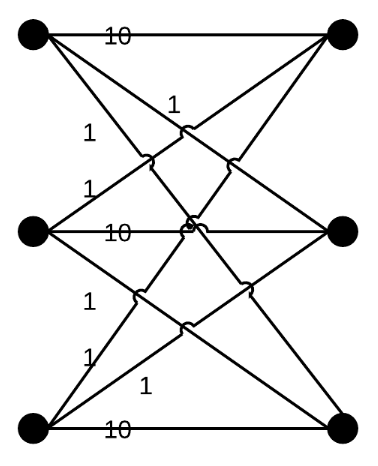
\includegraphics[width=50mm]{grapha.png}


\problem{Problem 4.} 
\problempart{a} Fix a vertex $i \in L$ and let the event
\[
A_j = \{\text{vertex } i \text{ is matched with vertex } j \in R\}
\] 
Let's call a vertex matched if the edge $(i,j)$ is in the output of the stateless rounding procedure. Then 
\[
P(\{\text{vertex } i \text{ is matched}\}) = P( \bigcup_{j\in R} A_j )
\]
For a single event $A_k$ we have that 
\[
P(A_k) = x_{ik}z_k^{-1}
\]
Because the events $A_k$ are not independent
\end{document}
